
In dieser Versuchsaufgabe wird bei kurzgeschlossener Sekundärwicklung die Eingangsspannung mit Hilfe eines Stelltransformators
so weit erhöht, bis der Nennstrom fließt.
In diesem Versuch sind die Eisenverluste vernachlässigbar klein,
Mit dem Leistungsmesser werden bei Kurzschluss somit die Kupferverluste  gemessen.

\par 
Die verwendete Messschaltung ist unten Abbgebildet.  \par
\begin{figure}[h]
    \centering
    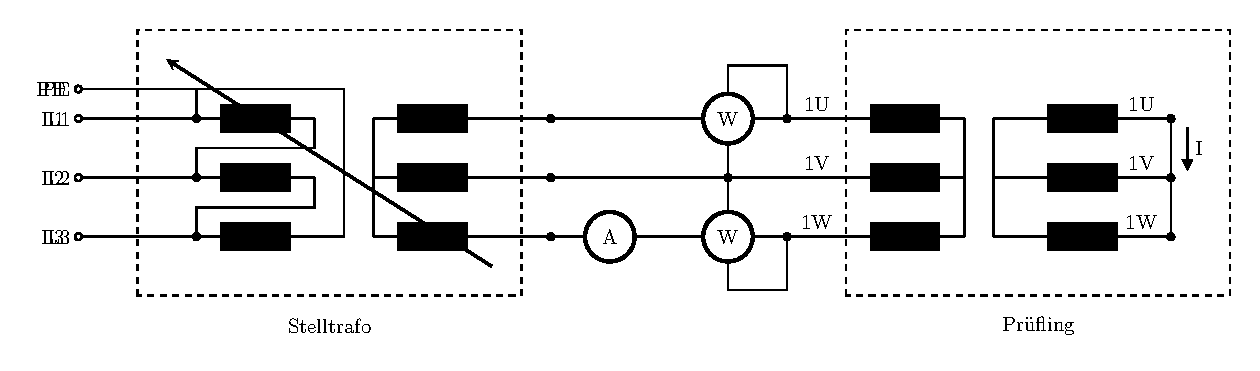
\includegraphics[width=0.95\textwidth]{fig/kz_mess.pdf}
    \caption{Messschaltung Kurzschluß}
    \label{fig:my_label}
 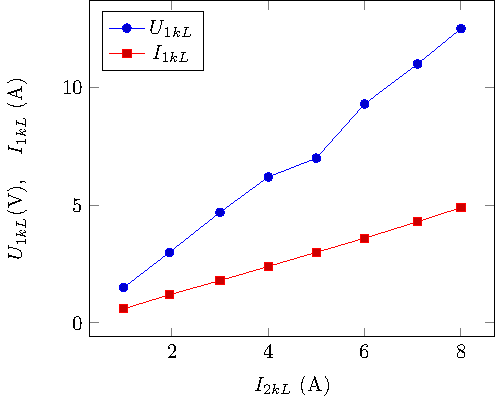
\includegraphics{fig/kz.pdf}
    \caption{Kurzschlussspannung und primärseitiger Kurzschlußstrom in Abhängigkeit von sekundärseitigem Kurzschlußstrom}
\end{figure}

\begin{align*}
\cos \phi_k &= \frac{P_k}{\sqrt{3}U_{1kL} \cdot I_{1k\varphi}}\\
&= \frac{75}{\sqrt{3}\cdot 4.9 \cdot 12.5} \\
&= 0.707\\
    Z_k &= \frac{V}{I}\\
    & = \SI{1.56}{\ohm}\\
    R_{k} &= \frac{P}{3 \cdot I_{\varphi}^2} = Z \cdot \cos \phi\\
    &=1.56 \cdot 0.707 \\
    &= \SI{1.04}{\ohm}\\
   X_k &= \SI{1.18}{\ohm}\\
    u_k &= \frac{U_{1k}}{U_{1B}}\cdot 100 \% \\
    &= \frac{12.5}{400}\cdot 100 \% \\
    & = \SI{3.125}{\percent}
\end{align*}
\begin{align*}
    R^\prime_2 &= \text{Ü}^2 \cdot R_1\\
    &= 1.73^2 \cdot 0.28 = \SI{0.83}{\ohm} \\ 
    X_k &= X_{\sigma 1} +   X_{\sigma 1} \cdot \frac{ R^\prime_2 }{R_1}\\
    X_{\sigma 1} &= \dfrac{X_k}{1+\dfrac{ R^\prime_2 }{R_1}}\\
     X_{\sigma 1} &= \dfrac{1.18}{1+\dfrac{0.83}{0.61}}\\
     &= \SI{0.5}{\ohm}\\
      X^\prime_{\sigma 2} &= \SI{0.68}{\ohm}
\end{align*}

\begin{figure}[H]
    \centering
    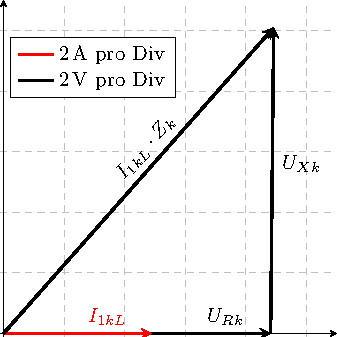
\includegraphics{fig/phasor_short.pdf}
    \caption{Caption}
    \label{fig:open}
\end{figure}